%%%% début de la page
\teteSndMouv

\nomPrenomClasse
\titreActivite{Forces d'interaction gravitationnelle}

\begin{objectifs}
  \item Connaître la force d'interaction gravitationnelle
\end{objectifs}

\pasCorrection{
  \begin{tableauCompetences}
    COM & Travailler en groupe, échanger entre élèves. \\
  \end{tableauCompetences}
}


%%
\begin{doc}{Force d'interaction gravitationnelle}{doc:A5_interaction_gravitationnelle}
  \chevron Tous les corps qui possèdent une masse s’attirent entre eux : c’est l’attraction gravitationnelle.
  \begin{importants}
    On modélise l'attraction gravitationnelle exercée par le corps $A$ sur le corps $B$ par une force représentée par un vecteur $\vvFAsurB$ :
    
    \vspace*{-12pt}
    \begin{wrapfigure}[6]{r}{0.4\linewidth}
      \vspace*{-10pt}
      \begin{tikzpicture}
  % corps A
  \tikzCercle[gray!50!white] (0, 0) {20}
  \tikzLabel(-1.2, 0) {$m_A$}
  \tikzPointLabel(0,0) {$A$}
  % corps B
  \tikzCercle[gray!50!white] (4, 2) {20}
  \tikzLabel(2.8, 2) {$m_B$}
  \tikzPointLabel(4, 2) {$B$}
  % force et distance
  \tikzVecteur(4, 2) (-1.75, -0.875) {$\vvFAsurB$} [left]
  \tikzVecteur*(0.5, -1) (4, 2) {}
  \tikzLabel(2.5, -0.5) {$d$}
\end{tikzpicture}
    \end{wrapfigure}
    \phantom{b}
    
    \begin{listePoints}
      \item \important{Point d'application} : centre du corps $B$
      \item \important{Direction} : la droite $AB$.
      \item \important{Sens} : de $B$ vers $A$ (force attractive).
      \item \important{Valeur} : 
    \end{listePoints}
    \begin{center}
      $\FAsurB =$ \texteTrouLignes{$G\times \dfrac{m_A \times m_B}{d^2}$}
    \end{center}
      
    Dans la formule de la valeur de la force, les masses s'expriment en kilogramme (\unit{\kg}),
    la distance en mètre (\unit{\m}) et
    la \important{constante universelle de gravitation $\mathbf{G}$} en newton mètre carrée par kilogramme carrée (\unit{\newton \m\squared \per\kg\squared}).
    Sa valeur (à connaître) est 
    \begin{center}
      $G =$ \texteTrou*{$\qty{6,67e-11}{\newton \m\squared \per\kg\squared}$}
    \end{center}
  \end{importants}
\end{doc}

%%%%
\numeroQuestion Compléter le document \ref{doc:A5_interaction_gravitationnelle}.


\question{
  Donner des exemples d'actions mécaniques qu'on rencontre dans la vie quotidienne.
}{
  Faire du vélo, tenir un stylo, porter son sac, tourner un guidon, etc.
}[5]

\question{
  Est-ce que ce sont des actions de contact, ou à distance ?
}{
  Ce sont des actions de contact, il faut toucher les objets pour agir sur eux, alors que l'interaction gravitationnelle est une action à distance.
}[2]


%%%%
\begin{doc}{Satellite Hubble}{doc:A5_satellite_hubble}
  \begin{wrapfigure}{r}{0.3\linewidth}
    \vspace*{-24pt}
    \centering
    \image{1}{images/mecanique/hubble}
  \end{wrapfigure}
  
  Le satellite Hubble est un satellite de masse $m_H = \qty{1,1e4}{\kg}$ conçu par la NASA avec une  participation de l'Agence spatiale européenne, l'ESA.
  
  Le satellite est attirée par la terre : il est en chute libre permanente.
  Le satellite est opérationnel depuis 1990 et tourne autour de la Terre en \qty{96}{\min}.
  Vu depuis le centre de la Terre, il a un mouvement circulaire uniforme à une altitude \important{$\mathbf{h = \qty{590}{\km}}$.}
  
  Ce satellite contient un télescope qui permet d’observer les étoiles et objets de l’univers depuis l’espace !
\end{doc}

\mesure 
Sur le schéma ci-dessous, représenter la force d’interaction gravitationnelle $F_{T/H}$ exercée par la Terre $T$ sur le satellite Hubble $H$.
La Terre est assimilée à une boule de rayon $R_T = \qty{6370}{\km}$ et de masse $M_T = \qty{5,97e24}{\kg}$.
\smallskip

\separationBlocs{
  \centering
  \begin{tikzpicture}
    % Satellite
    \tikzCercle[white] (0, 0) {80} [couleurSec]
    \tikzLabel(2.82, 0) {$H$} (3.2, 0) 
    % Terre
    \tikzCercle[couleurSec!30] (0, 0) {60} [couleurSec]]
    \tikzLabel(0, 0) {$T$}
    % Distance d
    \tikzVecteur*(0, 0) (-2.8, 0) {$d$} [below right]
    % Rayon de la Terre
    \tikzVecteur*(0, 0) (-0.54, -2.05) {}
    \tikzLabel*(0.3, -1) {$R_T$}
    % Hauteur du satellite
    \tikzVecteur*(-0.54, -2.05) (-0.18, -0.68) {}
    \tikzLabel*(-1.1, -2.2) {$h$}
  \end{tikzpicture}
  
  \legende{Schéma du satellite Hubble $H$ autour de la Terre $T$, les distances ne sont pas à l'échelle.}
}{
  \centering
  \begin{tikzpicture}
    \tikzCercle[white] (0, 0) {80} [couleurSec]
    \tikzLabel(2.82, 0) {$H$} (3.2, 0)
    \tikzCercle[couleurSec!30] (0, 0) {73.22} [couleurSec]]
    \tikzLabel(0, 0) {$T$}
  \end{tikzpicture}
  
  \legende{Schéma avec les distances à l'échelle.}
}
\smallskip

\question{
  Donner la formule mathématique qui relie la valeur de la force $F_{T/H}$ et la masse du satellite $m_H$, la masse de la Terre $M_T$, la constante $G$ et la distance $d$.
}{
  \begin{equation*}
    F_{T/H} = G\times \dfrac{m_H \times M_T}{d^2}
  \end{equation*}
}[3]

\question{
  Exprimer $d$ en fonction de $R_T$ et $h$.
  Calculer la valeur de $d$ en mètre.
}{
  \begin{equation*}
    d = R_T + h
  \end{equation*}
}[2]

\question{
  Calculer la valeur de $F_{T/H}$.
}{
  \begin{equation*}
    F_{T/H} = G\times \dfrac{m_H \times M_T}{d^2}
    = \qty{6,67e-11}{\newton \m\squared \per\kg\squared} 
      \times \dfrac{\qty{1,1e4}{\kg}
      \times \qty{5,97e24}{\kg}}{(\num{6,37e6} + \num{590e3})^2\unit{\km\squared}}
    = \qty{9,04e4}{\newton}
  \end{equation*}
}[5]